\documentclass[ngerman,a4paper]{texmf/tex/latex/mathscript/mathscript}
\usepackage{texmf/tex/latex/mathoperators/mathoperators}

\title{\textbf{Interpolation der \person{Runge}-Funktion und anderer Funktionen mit Octave}}
\author{\person{Henry Haustein}, \person{Lars Ortscheidt}}

\begin{document}
\maketitle
	
\tableofcontents
\pagebreak
	
\section{Interpolation der \person{Runge}-Funktion}	
	\begin{align}
		f(x) &= \frac{1}{1+25x^2}\notag \\
		f' (x) &= -\frac{50x}{625x^4+50x^2+1}\notag
	\end{align}
	
	\subsection{Berechnung der Splines}
	\subsubsection{Polynomsplines aus $\mathcal{S}_1^0(\Delta)$}
	
	Eine Polynomspline $s\in\mathcal{S}_1^0(\Delta)$ ist eine affin lineare Funktion, das heißt er hat die Form $s(x)=mx+n$ mit Anstieg $m$ und $y$-Achsenverschiebung $n$. 
	
	Die Interpolationsfunktion $g_N$, mit $N+1$ Stützstellen, besteht nun also aus Splines $s_i\in\mathcal{S}_1^0(\Delta)$, wobei für jeden Spline gilt:
	\begin{align}
		\text{Definitionsbereich: } & [x_i,x_{i+1}] \notag \\
		m_i =& \frac{f_{i+1}-f_i}{x_{i+1}-x_i}\notag \\
		n_i =& f_i \notag
	\end{align} 
	wobei $x_i$ die Stützstellen und $f_i$ die Stützwerte sind. Dabei läuft $i$ von $0$ bis $N-1$.
	
	Der Quelltext für Octave sieht dann so aus:
\begin{lstlisting}
runge = @(x) 1./(1+25*x.^2);
xreal = -1:0.01:1;

n = input('Anzahhl der Stuetzstellen - 1 := N: ');

%Schritweite h berechnen
h = 2/n
%Stuetzstellenvektor x berechnen
x = -1:h:1;

for i=1:n+1
 %Stutzwertevektor f berechnen
 f(i) = runge(x(i));
endfor

for i=1:n
 %Anstiege m_i berechnen
 m(i) = (f(i+1)-f(i))./(x(i+1)-x(i));
 %Achsenabschnitte n_i berechnen
 n(i) = f(i);
endfor

plot(x, f, "-;Interpol.;", xreal, runge(xreal), "-;Rungefkt.;")
\end{lstlisting}

	Das Interessante hierbei ist, dass die berechneten Werte in den Arrays \texttt{m} und \texttt{n} gar nicht für die Interpolation gebraucht werden - die Funktion \texttt{plot} interpoliert automatisch linear, wenn man ihr die Stützstellen und -werte übergibt.
	
	\begin{figure}[h]
		\centering
		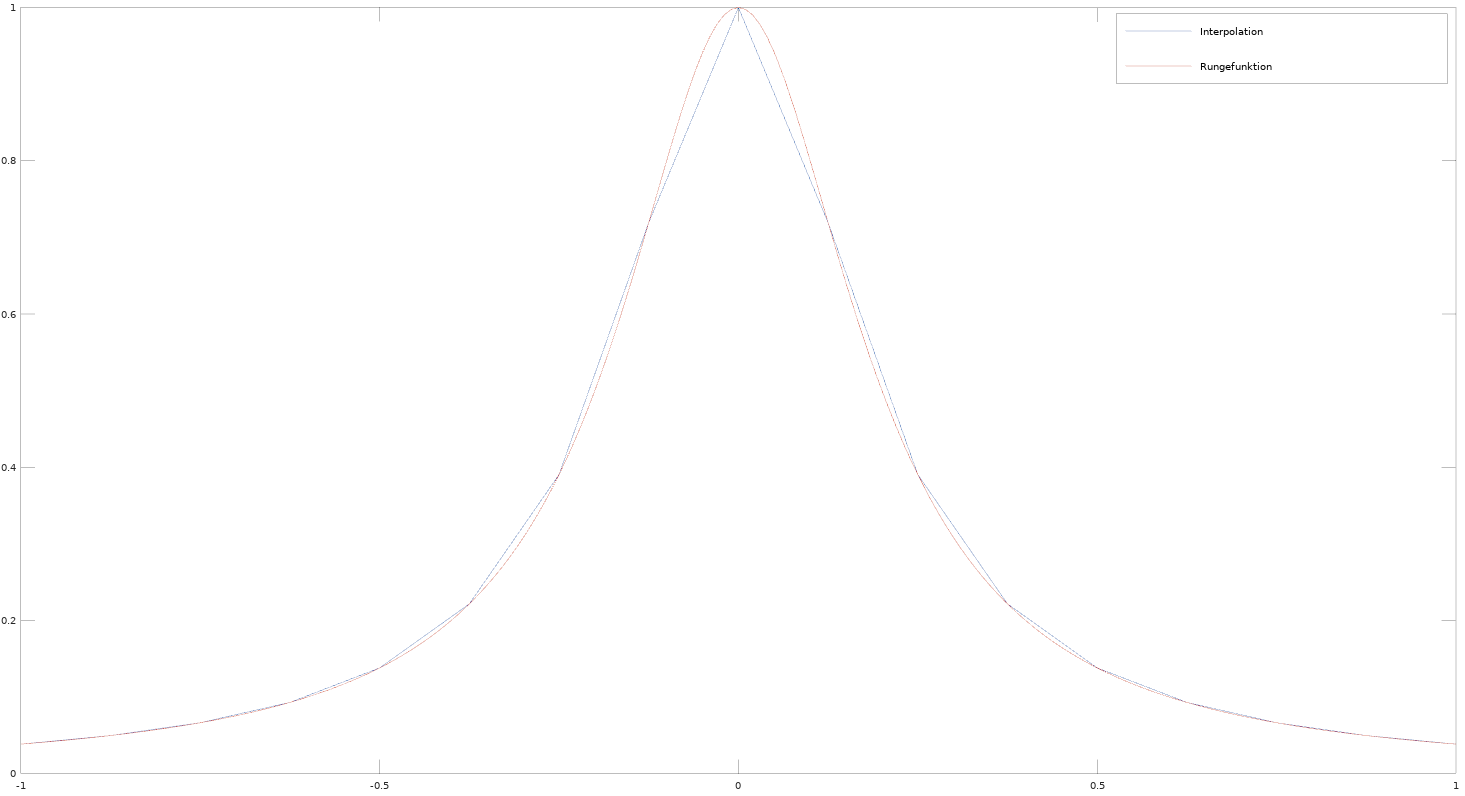
\includegraphics[width=0.9\textwidth]{images/Runge_lineare_Interpolation.png}
		\caption{lineare Splineinterpolation mit $N=16$}
	\end{figure}

	\begin{figure}[h]
		\centering
		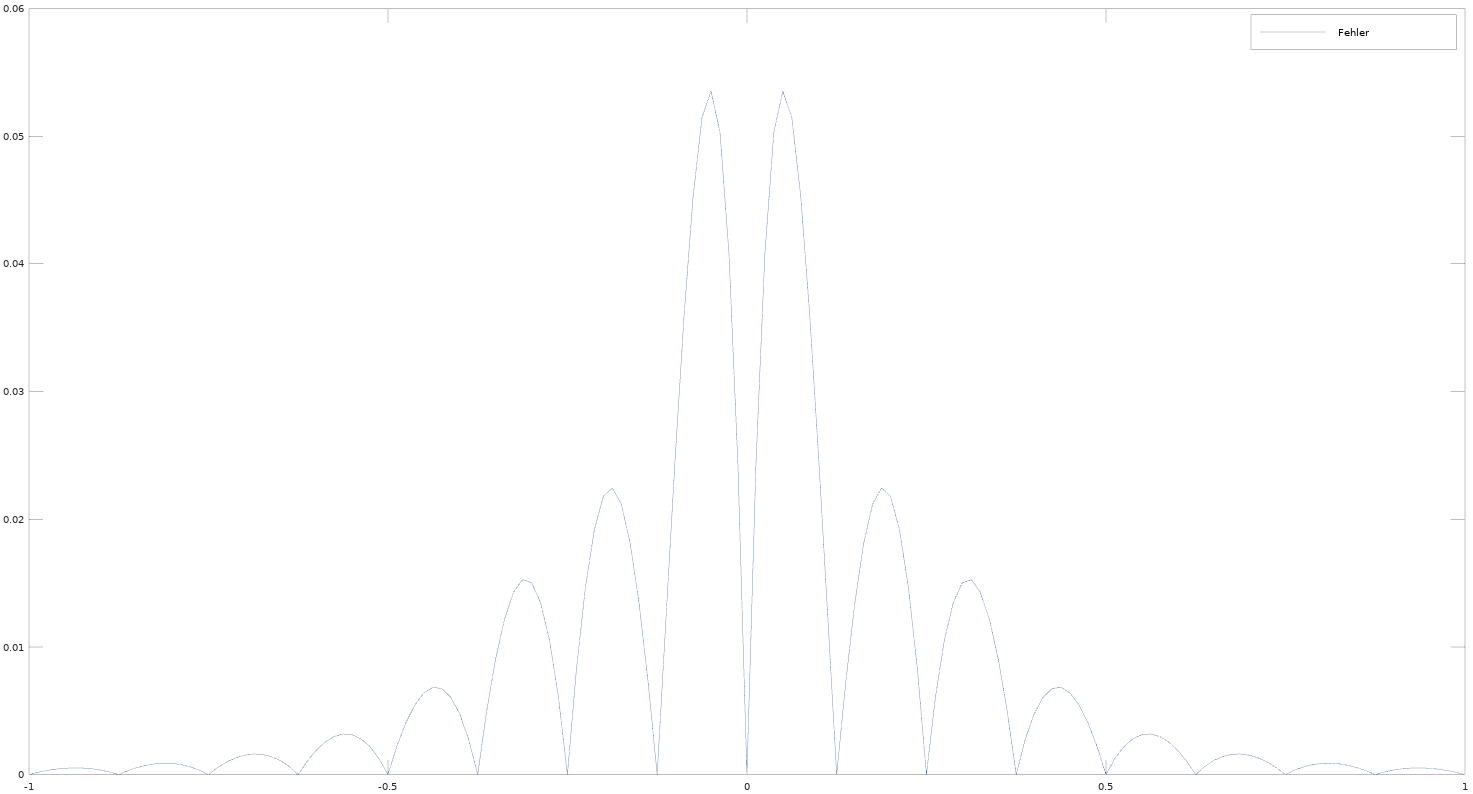
\includegraphics[width=0.9\textwidth]{images/Runge_lineare_Interpolation_Fehler.png}
		\caption{Fehler bei linearer Splineinterpolation mit $N=16$}
	\end{figure}
	
	\subsubsection{Polynomsplines aus $\mathcal{S}_3^1(\Delta)$}
	
	\subsection{Fehlerbetrachtung}
	
	Da $\Delta_M$ zehnmal so fein wie $\Delta_N$ ist, bedeutet das, dass man für jeden Spline den Fehler in 10 Punkten in seinem Definitionsbereich berechnet.
	
	Bei linearer Interpolation kann man also deswegen den Fehler nach folgendem Muster ausrechnen:
	\begin{align}
		\text{Fehler} = \vert f(x) - (n + \text{Abstand zur nächsten Stützstelle}\cdot m) \vert \notag
	\end{align}
	wobei $n$ und $m$ zum jeweiligen Spline gehören und $x$ die Werte in $\Delta_M$ durchläuft. Da die Fehlerfunktion laut Aufgabenstellung an den Stützstellen der Zerlegung $\Delta_M$ zu berechnen ist, lässt sich der nachfolgende Code auch für die Abschätzung des Fehlers (der auch an den Stützstellen von $\Delta_M$ gesucht ist) wiederverwenden. Der Quelltext dazu sieht folgendermaßen aus:
\begin{lstlisting}
M = 10 * N
h_neu = 2/M
x_Fehler = -1:h_neu:1;

k = 1;
for i=1:N
 %in jedem dieser Durchlauufe ist der Spline-Abschnitt der Selbe
 for j=1:10
  y_Fehler(k) = abs(runge(x_Fehler(k)) - ...
   (n(i) + abs(abs(x_Fehler(k)) - abs(x(i))) * m(i)));
  k = k + 1;
 endfor
endfor

%Fehler an letzter Stuetzstelle ist 0
y_Fehler(k) = 0;

plot(x_Fehler, y_Fehler, "-; Fehler;")

% maximaler Fehler E
E = max(y_Fehler)
\end{lstlisting}
	
	\subsection{Diskussion der Ergebnisse}
	
	Der maximale Fehler $E(h_N)$ für $N=N_k=4\cdot 2^k$ mit $k=0,...,4$ beträgt:
	\begin{center}
		\begin{tabular}{ll|l}
			$k$ & $N$ & $E(h_N)$ \\
			\hline
			0 & 4 & 0.17872 \\
			\hline
			1 & 8 & 0.063128 \\
			\hline 
			2 & 16 & 0.053536 \\
			\hline 
			3 & 32 & 0.020652 \\
			\hline 
			4 & 64 & 0.0058496 \\
		\end{tabular}
	\end{center} 


\section{Interpolation der anderen Funktion}
	\begin{align}
		f(x) &= \left( 1+\cos\left(\frac{3}{2}\pi x \right) \right)^{\sfrac{2}{3}}\notag \\
		f'(x) &=-\frac{\pi\sin\left(\frac{3}{2}\pi x\right)}{\sqrt[3]{1+\cos\left(\frac{3}{2}\pi x \right)}}\notag
	\end{align}
	
	\subsection{Berechnung der Splines}
	\subsubsection{Polynomsplines aus $\mathcal{S}_1^0(\Delta)$}
	
	\subsubsection{Polynomsplines aus $\mathcal{S}_3^1(\Delta)$}
	
	\subsection{Fehlerbetrachtung}
	
	\subsection{Diskussion der Ergebnisse}
\end{document}
